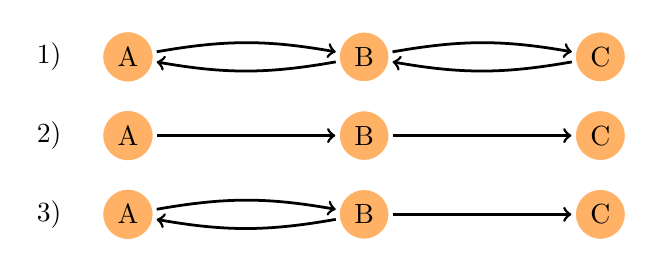
\begin{tikzpicture}
\tikzstyle{node_style} = [circle, draw=white, ultra thick, fill=orange!60]
\tikzstyle{edge_style} = [->, black, line width=1]
    \node[node_style] (v1) at (0,2) {A};
    \node[node_style] (v2) at (3,2) {B};
    \node[node_style] (v3) at (6,2) {C};

    \draw[edge_style] (v1) edge [bend left=10] (v2);
    \draw[edge_style] (v2) edge [bend left=10] (v1);
    \draw[edge_style] (v2) edge [bend left=10] (v3);
    \draw[edge_style] (v3) edge [bend left=10] (v2);

    \node[node_style] (v21) at (0,1) {A};
    \node[node_style] (v22) at (3,1) {B};
    \node[node_style] (v23) at (6,1) {C};

    \draw[edge_style] (v21) edge [] (v22);
    \draw[edge_style] (v22) edge [] (v23);

    \node[node_style] (v31) at (0,0) {A};
    \node[node_style] (v32) at (3,0) {B};
    \node[node_style] (v33) at (6,0) {C};

    \draw[edge_style] (v31) edge [bend left=10] (v32);
    \draw[edge_style] (v32) edge [bend left=10] (v31);
    \draw[edge_style] (v32) edge [] (v33);

    \node[] at (-1,2) {1)};
    \node[] at (-1,1) {2)};
    \node[] at (-1,0) {3)};
\end{tikzpicture}
